\documentclass{article}
\usepackage{afterpage}
\usepackage{float}
\usepackage{longtable}
\usepackage{graphicx}
\usepackage{pdflscape}
\usepackage[numbers,sort&compress]{natbib}
\usepackage{psfrag}

\usepackage{amsmath}
\usepackage{amsfonts}
\usepackage{graphicx}
\usepackage{nicefrac}
\usepackage{graphicx}
\usepackage{caption}
% \usepackage{subcaption}
\usepackage{subfigure}
% \usepackage{algorithm}
% \usepackage{paralist}
% % \usepackage[geometry]{ifsym}
\usepackage{rotating}
%
\newcommand{\uu}[1]{\boldsymbol #1}
\usepackage{listings}
\usepackage{xcolor}
\lstset{language=C++,
                keywordstyle=\color{blue},
                stringstyle=\color{red},
                commentstyle=\color{green},
                morecomment=[l][\color{magenta}]{\#}
}
\begin{document}

\begin{itemize}
    \item $\ell$: mesh level
    \item DoF: total degrees of freedom for the 4 by 4 system
    \item time$_{\rm AV}$: average FGMRES solve time
    \item time$_{\rm P}$: total non-linear time (includes all matrix assembles and all matrix solves)
    \item it$_{\rm P}$: number of Picard iterations
    \item it$_{\rm AVb}$: average number of FGMRES iterations
\end{itemize}


\begin{table} \centering
    \begin{tabular}{lrrrrrll}
    \hline
    $\ell$ &     DoF &  time$_{\rm AV}$ &  time$_{\rm P}$ &  it$_{\rm P}$ & it$_{\rm AV}$ \\
    \hline
     4 &    3,556 &       0.133 &           0.738 & 3 & 12.3 \\
     5 &   13,764 &       0.732 &           3.189 & 3 & 12.0 \\
     6 &   54,148 &       5.451 &          20.576 & 3 & 12.0 \\
     7 &  214,788 &      23.184 &          85.028 & 3 & 12.3 \\
     8 &  855,556 &     128.636 &         452.934 & 3 & 12.3 \\
    \hline
    \end{tabular}
    \caption{Cavity Driven - Direct application of the preconditioner}
\end{table}

\begin{table} \centering
    \begin{tabular}{lrrrrrll}
    \hline
    $\ell$ &     DoF &  time$_{\rm AV}$ &  time$_{\rm P}$ &  it$_{\rm P}$ & it$_{\rm AV}$ \\
    \hline
     4 & 3,556 & 0.30 & 1.240 & 3 & 13.7 \\
     5 & 13,764 & 1.77 & 6.327 & 3 & 13.3 \\
     6 & 54,148 & 8.84 & 30.419 & 3 & 13.7 \\
     7 & 214,788 & 46.11 & 154.014 & 3 & 13.7 \\
     8 & 855,556 & 178.131 & 594.776 & 3 & 13.3\\

    \hline
    \end{tabular}
    \caption{Cavity Driven - Iterative application of the preconditioner}
\end{table}

\begin{figure}
    \centering

  \subfigure[Velocity Solution]{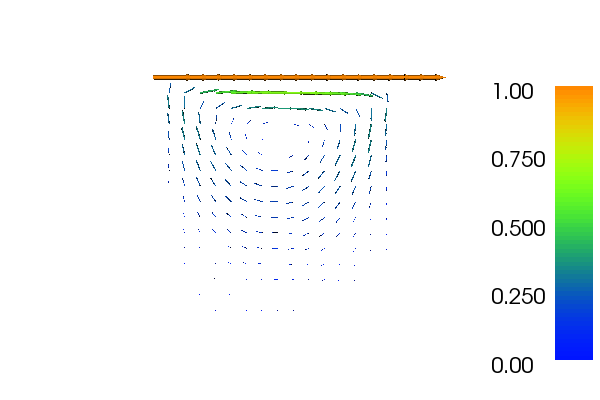
\includegraphics[width=60mm]{Figure/CDvelocity}}
  \subfigure[Magnetic Solution (normalised)]{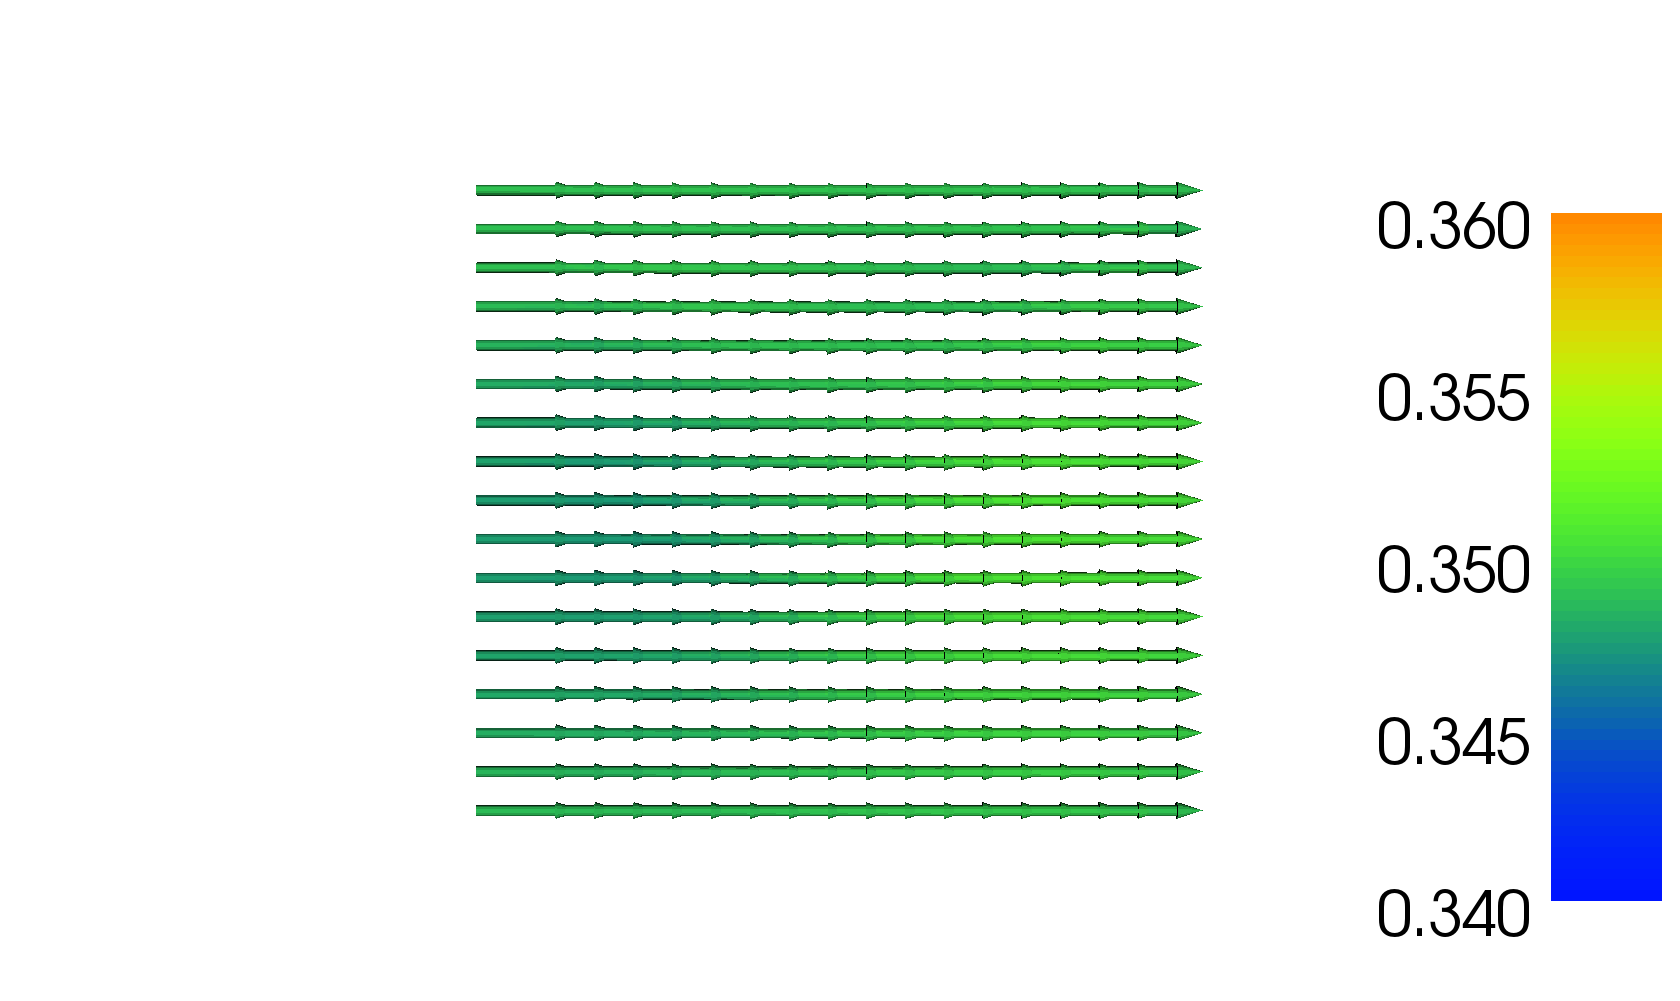
\includegraphics[width=60mm]{Figure/CDmagnetic}}
  \caption{Cavity Driven flow}
\end{figure}

\begin{table} \centering
    \begin{tabular}{lrrrrrll}
    \hline
    $\ell$ &     DoF &  time$_{\rm AV}$ &  time$_{\rm P}$ &  it$_{\rm P}$ & it$_{\rm AV}$ \\
    \hline
     4 &    3,140 & 0.091 & 0.579 & 3 & 13.3 & \\
     5 &   12,100 & 0.436 & 2.229 & 3 & 14.0 & \\
     6 &   47,492 & 2.246 & 10.196 & 3 & 14.0 & \\
     7 &  188,164 & 11.906 & 49.144 & 3 & 13.0 & \\
     8 &  749,060 & 49.345 & 201.360 & 3 & 11.3 & \\
    \hline
    \end{tabular}
    \caption{Flow over step - Direct application of the preconditioner}
\end{table}

\begin{table} \centering
    \begin{tabular}{lrrrrrll}
    \hline
    $\ell$ &     DoF &  time$_{\rm AV}$ &  time$_{\rm P}$ &  it$_{\rm P}$ & it$_{\rm AV}$ \\
    \hline
     4 &    3,140 & 0.308 & 1.640 & 4 & 19.2 \\
     5 &   12,100 & 1.484 & 7.345 & 4 & 19.0 \\
     6 &   47,492 & 7.269 & 25.259 & 3 & 17.0 \\
     7 &  188,164 & 30.333 & 103.745 & 3 & 16.7 \\
     8 &  749,060 & 187.996 & 652.892 & 3 & 15.0 \\

    \hline
    \end{tabular}
    \caption{Flow over step - Iterative application of the preconditioner}
\end{table}

\begin{figure}
    \centering

  \subfigure[Velocity Solution]{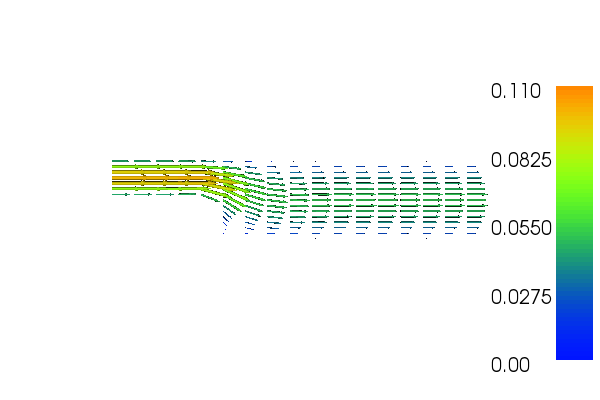
\includegraphics[width=60mm]{Figure/StepVelocity}}
  \subfigure[Pressure Solution]{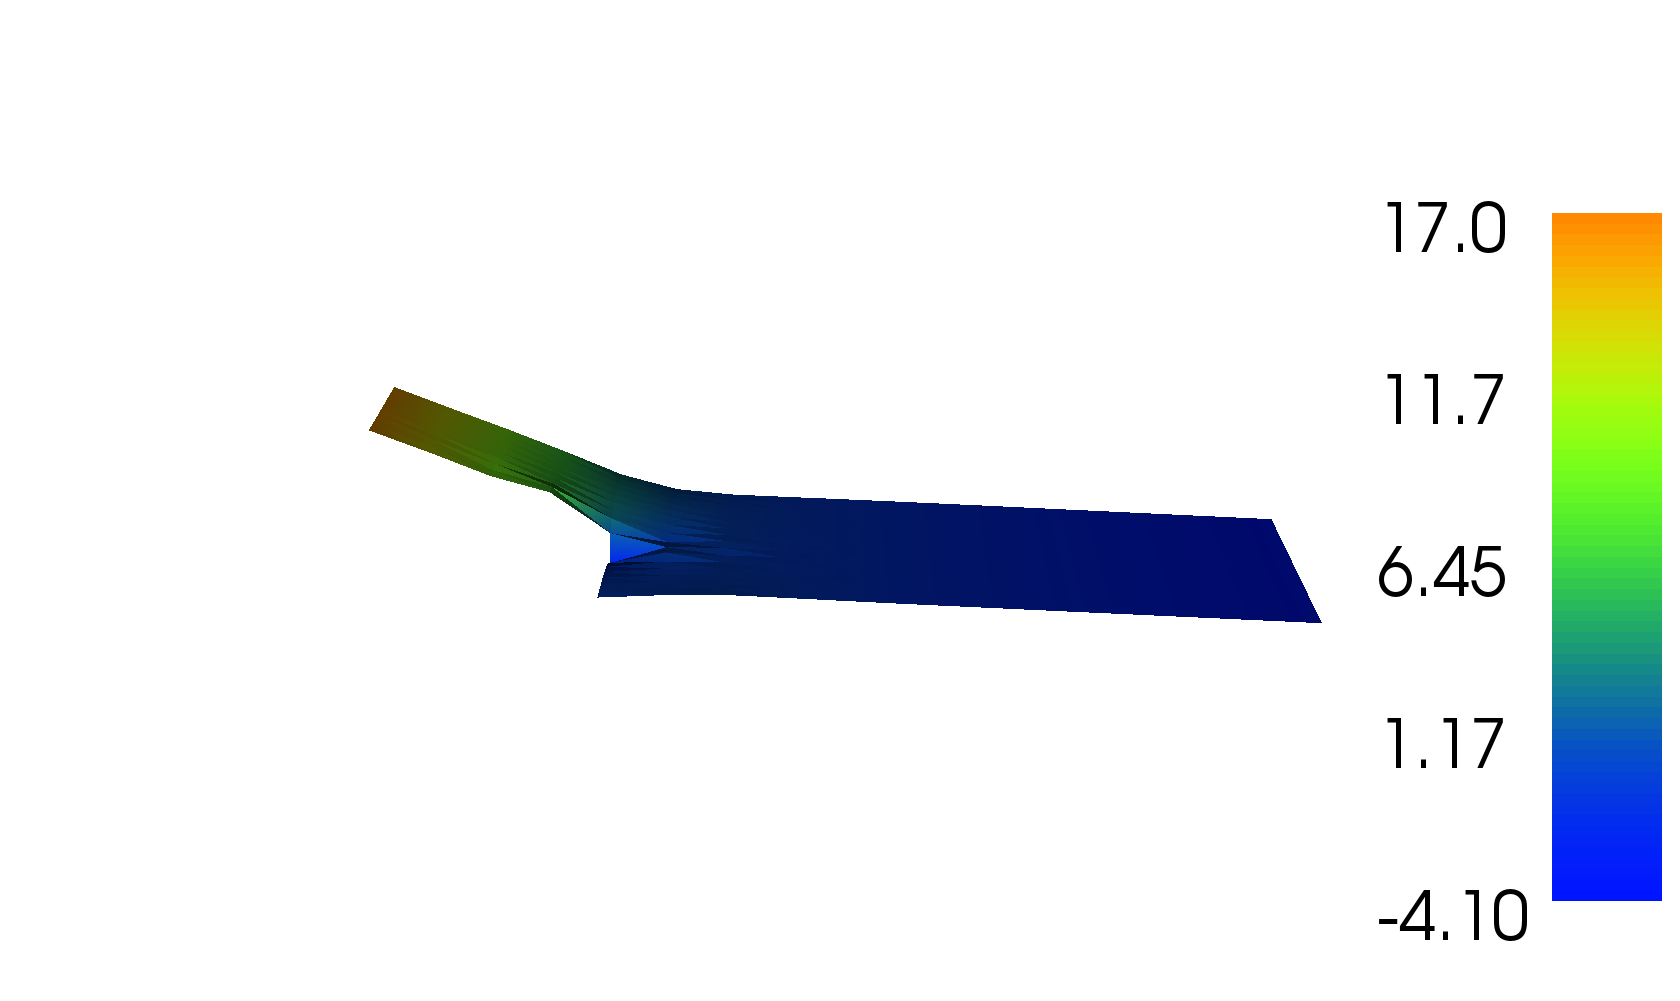
\includegraphics[width=60mm]{Figure/StepPressure}} \\
  \subfigure[Magnetic Solution]{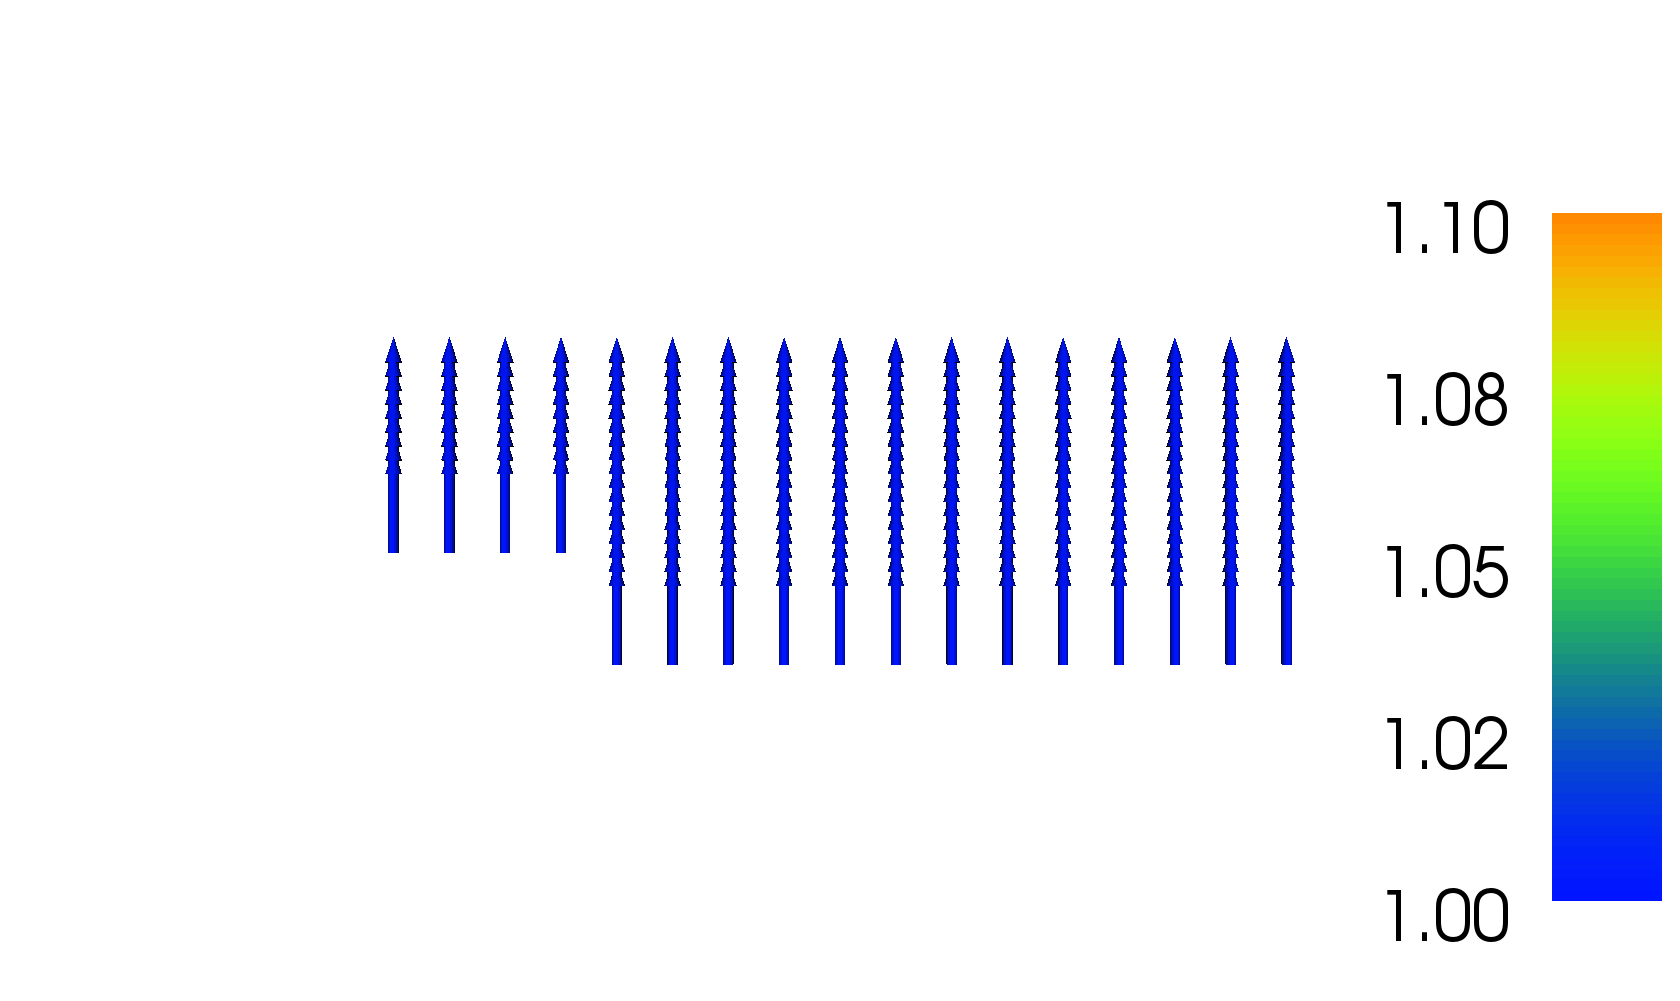
\includegraphics[width=60mm]{Figure/StepMagnetic}} \\
  \caption{Flow over step}
\end{figure}


\end{document}
